\documentclass[12pt,a4paper]{article}
\usepackage{task}

\newcommand{\contestName}{MateInfoUB}
\newcommand{\contestDates}{18 Mai 2025}
\newcommand{\contestPlace}{Facultatea de Matematic\v a-Informatic\v a}
\newcommand{\contestRound}{Runda Final\v a}
%\newcommand{\contestRound}{Rund\v a de Test}
\newcommand{\statementLanguage}{Rom\^ an\v a (Oficial)}
\newcommand{\taskShortName}{Moroi}


\definecolor{Brown}{cmyk}{0,0.81,1,0.60}
\definecolor{OliveGreen}{cmyk}{0.64,0,0.95,0.40}
\definecolor{CadetBlue}{cmyk}{0.62,0.57,0.23,0}
\definecolor{lightlightgray}{gray}{0.9}

\lstset{
% language=C++,                             % Code langugage
basicstyle=\ttfamily,                   % Code font, Examples: \footnotesize, \ttfamily
keywordstyle=\bfseries,        % Keywords font ('*' = uppercase)
commentstyle=\color{gray},              % Comments font
columns=flexible,
% numbers=left,                           % Line nums position
% numberstyle=\tiny,                      % Line-numbers fonts
% stepnumber=1,                           % Step between two line-numbers
% numbersep=5pt,                          % How far are line-numbers from code
% backgroundcolor=\color{lightlightgray}, % Choose background color
% frame=none,                             % A frame around the code
% tabsize=2,                              % Default tab size
% captionpos=b,                           % Caption-position = bottom
% breaklines=true,                        % Automatic line breaking?
% breakatwhitespace=false,                % Automatic breaks only at whitespace?
% showspaces=false,                       % Dont make spaces visible
% showtabs=true,                         % Dont make tabls visible
}


\setlength{\parskip}{0pt}

\begin{document}
% Tex fragment for task statement headers
% Usage:
%       % Defining parameters required for header
%       \newcommand{\contestName}{Name of the Contest Series}
%       \newcommand{\contestDates}{Month 1 -- 8 20XX}
%       \newcommand{\contestPlace}{City, Country}
%       \newcommand{\contestRound}{Day 1}
%       \newcommand{\statementLanguage}{en (US)}
%       \newcommand{\taskShortName}{task_short_name}
%       % Tex fragment for task statement headers
% Usage:
%       % Defining parameters required for header
%       \newcommand{\contestName}{Name of the Contest Series}
%       \newcommand{\contestDates}{Month 1 -- 8 20XX}
%       \newcommand{\contestPlace}{City, Country}
%       \newcommand{\contestRound}{Day 1}
%       \newcommand{\statementLanguage}{en (US)}
%       \newcommand{\taskShortName}{task_short_name}
%       % Tex fragment for task statement headers
% Usage:
%       % Defining parameters required for header
%       \newcommand{\contestName}{Name of the Contest Series}
%       \newcommand{\contestDates}{Month 1 -- 8 20XX}
%       \newcommand{\contestPlace}{City, Country}
%       \newcommand{\contestRound}{Day 1}
%       \newcommand{\statementLanguage}{en (US)}
%       \newcommand{\taskShortName}{task_short_name}
%       \input{header.tex}
%


%--------------------- tools ----------------------
\makeatletter
% \expandafter for the case that the parameter is given in a command
\newcommand{\escapeUnderscores}[1]{\expandafter\@repl@underscores#1_\relax}
\def\@repl@underscores#1_#2\relax{%
    \ifx \relax #2\relax
        % #2 is empty => finish
        #1%
    \else
        % #2 is not empty => underscore was contained, needs to be replaced
        #1%
        \textunderscore
        % continue replacing
        % #2 ends with an extra underscore so I don't need to add another one
        \@repl@underscores#2\relax
    \fi
}
\makeatother
% -------------------------------------------------

\vspace*{-3em}\hspace*{-.5cm}
\begin{tabular}{ccl}
    \hspace{1mm}
\includegraphics[width=2.2cm,valign=b]{logo.jpeg}
    & 
    \begin{minipage}[b]{10cm}
        \setlength{\baselineskip}{1.05\baselineskip}
        \sffamily
        \makebox[0pt][l]{\bfseries \large \contestName}  \\
        \contestDates \\ 
        \contestPlace
    \end{minipage}
    & 
    \begin{minipage}[b]{3.7cm}
        \begin{flushright}
            \makebox[0pt][r]{\ttfamily \bfseries \large \escapeUnderscores{\taskShortName}}  \\[.2em]
            \sffamily
            \contestRound \\
            \statementLanguage
        \end{flushright}
    \end{minipage}
\end{tabular} 
\hrule height .06em
%


%--------------------- tools ----------------------
\makeatletter
% \expandafter for the case that the parameter is given in a command
\newcommand{\escapeUnderscores}[1]{\expandafter\@repl@underscores#1_\relax}
\def\@repl@underscores#1_#2\relax{%
    \ifx \relax #2\relax
        % #2 is empty => finish
        #1%
    \else
        % #2 is not empty => underscore was contained, needs to be replaced
        #1%
        \textunderscore
        % continue replacing
        % #2 ends with an extra underscore so I don't need to add another one
        \@repl@underscores#2\relax
    \fi
}
\makeatother
% -------------------------------------------------

\vspace*{-3em}\hspace*{-.5cm}
\begin{tabular}{ccl}
    \hspace{1mm}
\includegraphics[width=2.2cm,valign=b]{logo.jpeg}
    & 
    \begin{minipage}[b]{10cm}
        \setlength{\baselineskip}{1.05\baselineskip}
        \sffamily
        \makebox[0pt][l]{\bfseries \large \contestName}  \\
        \contestDates \\ 
        \contestPlace
    \end{minipage}
    & 
    \begin{minipage}[b]{3.7cm}
        \begin{flushright}
            \makebox[0pt][r]{\ttfamily \bfseries \large \escapeUnderscores{\taskShortName}}  \\[.2em]
            \sffamily
            \contestRound \\
            \statementLanguage
        \end{flushright}
    \end{minipage}
\end{tabular} 
\hrule height .06em
%


%--------------------- tools ----------------------
\makeatletter
% \expandafter for the case that the parameter is given in a command
\newcommand{\escapeUnderscores}[1]{\expandafter\@repl@underscores#1_\relax}
\def\@repl@underscores#1_#2\relax{%
    \ifx \relax #2\relax
        % #2 is empty => finish
        #1%
    \else
        % #2 is not empty => underscore was contained, needs to be replaced
        #1%
        \textunderscore
        % continue replacing
        % #2 ends with an extra underscore so I don't need to add another one
        \@repl@underscores#2\relax
    \fi
}
\makeatother
% -------------------------------------------------

\vspace*{-3em}\hspace*{-.5cm}
\begin{tabular}{ccl}
    \hspace{1mm}
\includegraphics[width=2.2cm,valign=b]{logo.jpeg}
    & 
    \begin{minipage}[b]{10cm}
        \setlength{\baselineskip}{1.05\baselineskip}
        \sffamily
        \makebox[0pt][l]{\bfseries \large \contestName}  \\
        \contestDates \\ 
        \contestPlace
    \end{minipage}
    & 
    \begin{minipage}[b]{3.7cm}
        \begin{flushright}
            \makebox[0pt][r]{\ttfamily \bfseries \large \escapeUnderscores{\taskShortName}}  \\[.2em]
            \sffamily
            \contestRound \\
            \statementLanguage
        \end{flushright}
    \end{minipage}
\end{tabular} 
\hrule height .06em

\section*{Creaturi 4: Moroii}


\begin{center}
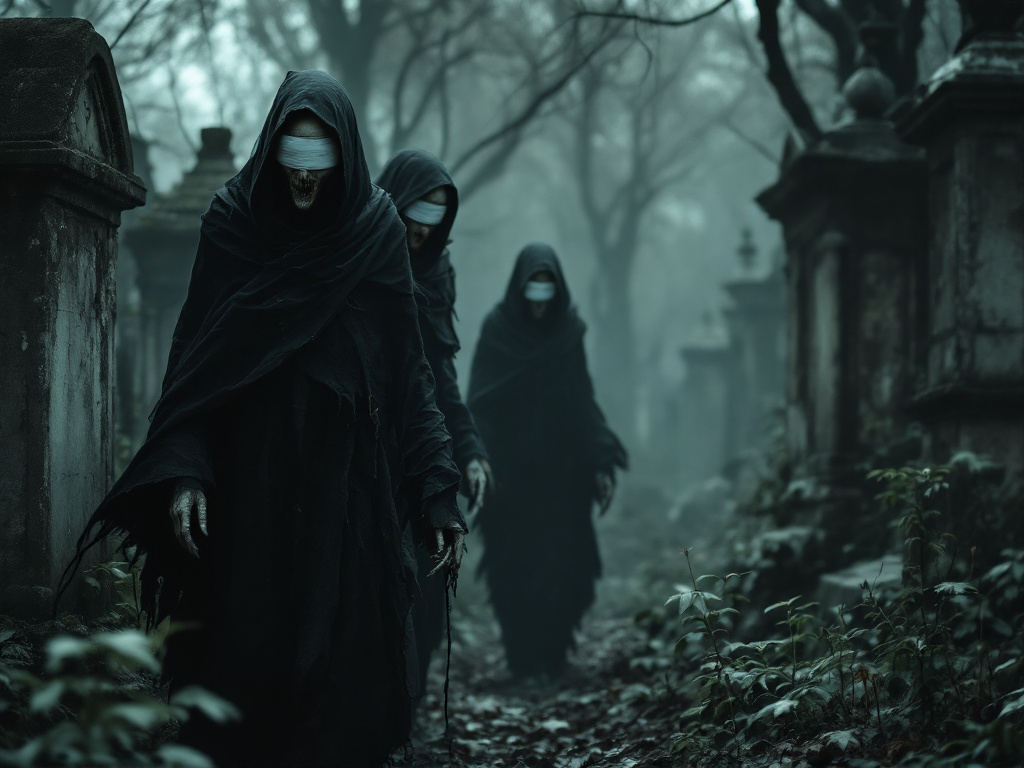
\includegraphics[scale=0.2]{moroi.jpg}
\end{center}

Legendele spun că în adâncul cimitirului \textit{"Umbrele Pierdute"}, moroii își fac simțită prezența, rătăcind printre morminte și așteptând să prindă vreun nefericit aventurându-se prin cimitirul abandonat după apusul soarelui.

\vspace{1em}

Din păcate, cum acest lucru nu se întâmplă foarte des, moroii se plictisesc, așa că au decis să joace de-a \textit{rătăcirea}.

\vspace{1em}

Cimitirul poate fi modelat ca un plan, cu X de la vest la est și Y de la sud la nord. Un moroi este așezat în centrul cimitirului la poziția $(0, 0)$, inițial îndreptat spre Est. După aceea, el primește o serie de instrucțiuni, care pot fi:

\begin{itemize}
    \item \texttt{"i"}: Înainte, moroiul înaintează o unitate în față.
    \item \texttt{"s"}: Stânga, moroiul se rotește cu 90 de grade spre stânga.
    \item \texttt{"d"}: Dreapta, moroiul se rotește cu 90 de grade spre dreapta.
    \item \texttt{"r"}: Rototol, moroiul se rototolește (se învârte) și alege o directie aleatoare din cele 4 posibile.
\end{itemize}


\vspace{1em}

Un moroi a urmat un set de instrucțiuni și a ajuns la poziția $(x, y)$. Acum se întreabă care este distanța maximă la care se poate afla de poziția inițială. Ajutați-l! 

Distanța de la $(0, 0)$ la $(x, y)$ este $|x| + |y|$.

\subsection*{Date de intrare}

Pe prima linie se găsește numărul $N$, numărul de instrucțiuni.
Pe următoarea linie se află un șir de caractere de lungime $N$, care reprezintă, în ordine, operațiile efectuate de moroi.

\subsection*{Date de ieșire}

Pe unica linie afișati numărul cerut.

\subsection*{Constrângeri}

\begin{itemize}
    \item $1 \leq N \leq 10^5$.
    \item Se garantează că datele din input sunt corecte.
\end{itemize}


\subsection*{Subtask-uri}

\begin{enumerate}
    \item ($40$ de puncte) Moroiul nu are de efectuat niciun rototol.
    \item ($30$ de puncte) Moroiul are de efectuat maxim două rototoale.
    \item ($30$ de puncte) Nicio constrângere suplimentară.
\end{enumerate}

\subsection*{Exemplu}

\begin{tabular}{|@{}p{0.5\textwidth}@{}|@{}p{0.5\textwidth}@{}|}
\hline
\multicolumn{1}{|c|}{\bfseries Input Standard (\textit{cin})} &
\multicolumn{1}{c|}{\bfseries Output Standard (\textit{cout})} \\
\hline
\begin{textQuoteCell}
10
isisirdisi
\end{textQuoteCell} &
\begin{textQuoteCell}
3
\end{textQuoteCell} \\    
\hline
\begin{textQuoteCell}
59
dsisididdsiiiriirrssridrsssiiddisssiir
irdiisisriidisiiisisi
\end{textQuoteCell} &
\begin{textQuoteCell}
18
\end{textQuoteCell} \\    
\hline
\end{tabular}
\vspace{1em}

\subsection*{Explicație exemplu 1}

Parcusul care maximizează $|x| + |y|$ pentru moroi este următorul:

\begin{itemize}
    \item \texttt{i}: Din $(0, 0)$ merge în $(1, 0)$, îndreptat spre Est.
    \item \texttt{s}: Rămâne în $(1, 0)$, se îndreaptă spre Nord.
    \item \texttt{i}: Din $(1, 0)$ merge în $(1, 1)$, îndreptat spre Nord.
    \item \texttt{s}: Rămâne în $(1, 1)$, se îndreaptă spre Vest.
    \item \texttt{i}: Din $(1, 1)$ merge în $(0, 1)$, îndreptat spre Vest.
    \item \texttt{r}: Rămâne în $(0, 1)$, se îndreaptă spre Nord.
    \item \texttt{d}: Rămâne în $(0, 1)$, se îndreaptă spre Est.
    \item \texttt{i}: Din $(0, 1)$ merge în $(1, 1)$, îndreptat spre Est.
    \item \texttt{s}: Rămâne în $(1, 1)$, se îndreaptă spre Nord.
    \item \texttt{i}: Din $(1, 1)$ merge în $(1, 2)$.
\end{itemize}

Așadar, ajunge la o distanță de 3 față de origine.

\end{document}